%\documentclass{report}

%\usepackage{amssymb}
%\usepackage{amsfonts}
%\usepackage{amsmath}
%\usepackage{dsfont}
%\usepackage[a4paper, total={6in,8in}]{geometry}
%\usepackage{graphicx}
%\usepackage{float}
%\usepackage{natbib}
%\usepackage{hyperref}

%\graphicspath{{figures/}}

%\title{One mass}
%\author{Will Woolfenden}

%\begin{document}

\chapter{The single mass model}
\label{cha:onemass}

\section{Principles of the single-mass model}

\begin{figure}[h!]
	\centering
	\includegraphics[width=\linewidth]{figures/onemass.jpeg}
	\caption{
		Two dimensional schematic sketch of the single mass model.
		Fluid flow $V$ travels through the channel,
		and we are interested in the motion of the plate with mass $\mathrm{m}$.
	}
\end{figure}

\subsection{Derivation}

The first model we will study is taken from Theory and Measurement of Snores \citep{gavriely_jensen_1993}.
It models the inspiratory process, designed to investigate snoring as a symptom of obstructive sleep apnea.
The model proposes that the inspiratory path consists of first a region of the upper airway,
which has a given viscous resistance.
Then, there is a region of a channel between two walls of given area, where one wall is a suspended plate rather than being fixed in place.
The term we wish to investigate is $b$, which describes the positive displacement between the fixed wall and the suspended wall opposite.
Equivalently, $b$ models the glottal opening.
The walls themselves are assumed to be of equal dimensions, and behave such that the surfaces are always parallel to each other.
We impose that the plate may only move in the direction of $b$ which is the normal to its surface,
hence $b$ measures the only degree of freedom of the plate's motion.

%figure on diagram of the model

The oscillations in $b$ that may take place, depending on conditions, is the subject of our analysis.
In the original paper, the oscillations are regarded as snores,
whereas here they will be regarded as the production of phones.
The idea is the same, since the mathematical principles applied in the definition of the model are not exclusive in any way to particular studies of sleep apnea or the like.

Oscillations are the event where, given certain constraints, $b$ will exhibit periodic motion, regularly returning to an initial position. %maybe cite here
In the model provided, indefinite oscillations can very much be observed given the right conditions,
however it is important to be aware of some properties of the model,
namely the region in which our attention is focussed. Given physical attributes are associated with the model,
and so, for example, behaviours of $b$ when negative are ignored in the investigation.

There are three forces acting on the plate in the airway, which govern the motion we are investigating.
The plate is suspended in place by an elastic force $F_k$, namely a conventional Hooke spring with spring constant $k$.
This spring force suspends the plate such that it resists the closure of the airway,
so the tension force on the plate is acting tangent to the direction of positive displacement of the plate.

% schematic with opposing walls and illustration of spring direction.

Since the upper airway has a viscous resistance $R$ to the fluid flow,
this leads to a pressure drop in the airways. %TODO: Explain this
An internal increase in pressure would produce an outward force on the airway,
which in this model would be tangent to the positive displacement direction.
Since there is instead a \textit{decrease} in pressure, an inward force is resultant,
in the direction tangent to the negative displacement. We label this force as $F_p$.
Pressure itself is the force per unit area,
so the value of the force $F_p$ is the pressure multiplied by the surface area of the plate.

Bernoulli's equation for a steady flow gives us a relationship between pressure and fluid velocity.
Assuming no body forces, the potential $\Omega$ is zero,
so we can consider the flow local to the lung, and the flow near the opening.
Formally, this can be represented by the equation
\begin{equation}
    \left.\left(\frac{1}{2}|\mathbf{u}|^2 + \int \frac{\mathrm{d}p}{\rho}\right)\right|_\mathrm{in} = \left.\left(\frac{1}{2}|\mathbf{u}|^2 + \int \frac{\mathrm{d}p}{\rho}\right)\right|_\mathrm{out}
\end{equation}
This expression can be rearranged to find an expression for the pressure.
We would assume that the fluid velocity is zero local to the lung (in),
being driven by the pressure.
Hence the pressure at the opening (out) is a function of the speed local to the opening,
and the forcing pressure at the lung.
Note that the term $|\mathbf{u}|^2/2$ is the fluid kinetic energy per unit mass.
We obtain the force $F_b$ by multiplying this pressure term by the cross-sectional area of the plate.
If this pressure is below atmospheric,
then the resulting force on the plate is acting inwards,
which is the same as $-F_b$ acting outwards.

The governing equation of the model is derived from Newton's second law.
Given that the plate has a mass $m$, we know the three forces acting on it,
and so the initial equation of motion can be expressed as
\begin{equation}
    m\frac{d^2 x}{dt^2} = F_e - F_p - F_b.
    \label{eqn:model_init}
\end{equation}
This is not the principal equation of the model,
since the terms should be nondimensionalised and normalised.
For example, $x$ measures displacement but it is not stated under what scale.
Furthermore, the terms for the forces are all products of pressure and their dimensional properties,
meaning they measure in units that would ideally be reduced.
We can normalise $x$ by defining $b = x/x_0$, where $x_0$ is an equilibrium position of the plate.
The forces can be nondimensionalised by dividing by the areas or volumes they are acting over.
We will further explore nondimensionalisation in the study of the two mass model.
Resultingly, we produce the governing equation for the positive displacement of the channel wall from collapse at $0$,
\begin{equation}
    \frac{d^2b}{dt^2} = 1 - q - b - \frac{\mu q^2}{2b^2}
    \label{eqn:master}
\end{equation}
where $\mu, q$ are parameters linked to the properties of the fluid flow.

%plan is to have this chapter just discuss individual properties of the model with analysis where relevant. Will include matrix method. Then in next chapter we introduce KE graphs in the phase-plane.

\subsection{Nonlinearity}

It is important to note the properties of Equation \ref{eqn:master} before developing analysis.
The equation itself is a second order, nonlinear, autonomous, inhomogeneous ODE.
The property of nonlinearity is due to the existence of the $\mu q^2/2b^2$ term.
Due to the equation being nonlinear, regular methods for solving ODEs are far less powerful,
and the properties of solutions are different to regular linear ODEs.
Most importantly, while linear ordinary differential equations often possess unique solutions subject to boundary or initial conditions,
the same does not apply in the case of nonlinear equations.

We will first demonstrate the implications of nonlinearity by attempting methods suitable for linear ODEs,
in which we do not expect to solve the ODE but instead use for demonstration.
Note the absence of the $db/dt$ term in the governing equation.
We can attempt the method of reduction by proposing a substitution $v=db/dt$ and forming a first order ODE.
First, note that
\begin{equation}
    \frac{dv}{dt} = \frac{dv(b(t))}{dt} = \frac{dv}{db}\frac{db}{dt} = \frac{dv}{db}v,
\end{equation}
and hence,
\begin{equation}
    v \frac{dv}{db} = 1 - q - b - \frac{1}{2}\mu q^2\left( \frac{1}{b^2} \right).
\end{equation}
Assuming we can separate the variables, we can write an indefinite integral equation and obtain an expression for $v$, namely
\begin{equation}
    \begin{aligned}
        \int v~dv &= \int \left(1 - q - b - \frac{1}{2}\mu q^2 b^{-2} \right) db \\  %TODO: edits. separate all this mess.
        v^2 &= \left(\frac{db}{dt}\right)^2 = 2b(1-q) - {b^2} + \mu q^2 b^{-1} + C_1, %we have integrated AND multiplied by 2.
    \end{aligned}
    \label{eqn:first_order_reduction}
\end{equation}
obtaining a constant of integration $C_1$.
We now have a first order differential equation on $b$, %however we can't solve it because no
but this equation is even harder to reduce or even solve, as we only have the form $v^2 = g(b)$,
where the first derivative is expressed explicitly but not linearly.
Therefore, statements of existence and uniqueness for solutions of ODEs,
which we are accustomed to,
do not hold in the situation where the differential equation is non-linear.

We could have deduced this from the explicit form of Equation \ref{eqn:master},
but this section serves for illustration to aid the reader's understanding of why we cannot analytically solve this ODE.
Additionally, the equation of the form $v^2 = g(b)$ will be useful later.

\subsection{Properties of an autonomous system}

\begin{figure}[h!]
    \centering
    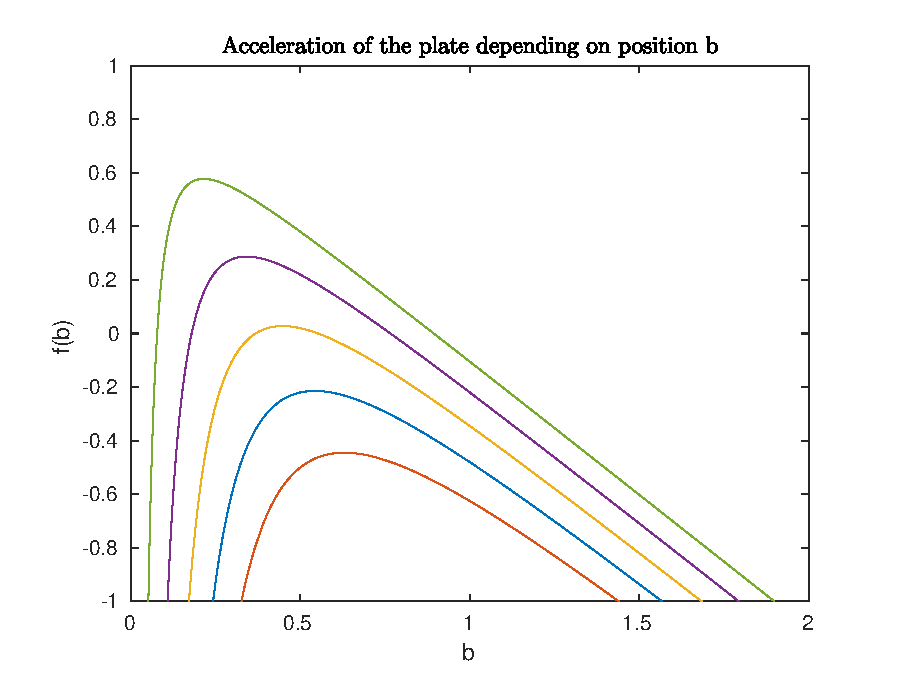
\includegraphics[width=0.5\linewidth]{figures/f_plot_mu_1_q_vary}
    \caption{A plot of the function $f(b) = 1-q-b-\mu q^2/2b^2$ where $\mu=1$, $q$ ranging from $0.1$ (orange) to $0.5$ (green).}
    \label{fig:acc_b_plot}
\end{figure}

\begin{figure}[h!]
	\centering
	\includegraphics[width=\linewidth]{figures/bifurcation_saddlenode}
	\caption{
		The convergence of the equilibrium solutions to a single point before annihilating. Computed by solving \(f(b)\) with Newton's method.
		The parameter \(q\) is the independent variable that governs the distance between the equilibria, while we have \(\mu\) fixed.
	}
	\label{fig:bifurcation}
\end{figure}
The reader may notice that the Equation \ref{eqn:master} is an autonomous ODE,
namely that the independent variable $t$ itself does not appear.
If we let $f$ be a function of $b$ equal to the right-hand side of the equation,
we can produce a plot of the behaviour of $f(b)$ against $b$.
The visualisation of $f(b)$ shows the acceleration on the plate given its position.
Since the equation is autonomous, $f$ is unchanging in time.
Figure \ref{fig:acc_b_plot} shows a plot of $f(b)= 1 - q - b - \mu q^2/2b^2$ against $b$.

We will introduce the concept of equilibrium solutions of the ODE,
being fixed-point solutions that tell us a lot of information about the behaviour of the model.
For example, later on we will construct an approximation to the ODE close to an equilibrium solution,
and this approximation will be linear.
An equilibrium solution is a zero of the function \(f(b)\), since all time derivatives of \(b(t)\) are zero if \(b\) is fixed.

This plot allows us to deduce some intuition about the behaviour of $b$.
At a point $b=b_0$, the function $f(b_0)$ is equal to the outward acceleration of the plate.
We can see that $f$ tends towards negative infinity both as $b\rightarrow 0$ and as $b\rightarrow\infty$,
and that for certain $\mu, q,$ there is a positive region of $f$.
Hence if $b$ is either small or large, it will accelerate to closure,
whereas for a range of intermediate values it may accelerate outwards instead.
It is possible under certain conditions for $b$ to behave similarly to a harmonic oscillator,
where its position and acceleration move back and forth reciprocally.

Note that the plot of $f(b)$ does not account for velocity.
Different initial conditions could cause $b$ to behave differently under the same acceleration.

We will start by analysing the properties of the $f(b)$ curve.
In order for there to exist a region of $f(b)$ that takes positive values,
the local maximum of $f(b)$ must be greater than zero.
We can take the derivative of $f(b)$,
\begin{equation}
    f'(b) = -1 + \frac{\mu q^2}{b^3}
\end{equation}
from which we can deduce that the maximum is located at the point where $b^3 = \mu q^2$.
If we plug this back into $f$, we can deduce the condition
\begin{align}
    f((\mu q^2)^{\frac{1}{3}}) & = 1 - q - (\mu q^2)^{\frac{1}{3}} - \frac{\mu q^2}{2(\mu q^2)^{\frac{2}{3}}} \\
                               & = 1 - q - \frac{3}{2}(\mu q^2)^{\frac{1}{3}}.
\end{align}
We want \(f((\mu q^2)^{1/3}) > 0 \). We can expand and rearrange to obtain an explicit expression, being
\begin{equation}
    \frac{(1-q)^3}{q^2} > \frac{27}{8}\mu
    \label{eqn:osc_condition}
\end{equation}
If Equation \ref{eqn:osc_condition} is satisfied,
then there exists a region of $f$ which is positive.
Hence if this condition is met then oscillations may occur. %% I feel this should be more rigorous - we haven't proved that this is the condition for oscillations to occur.
We have not yet provided the results to justify this statement, but later on we will provide more analysis on how the values of the parameters affect oscillations.
Further on, we will be regularly making the assumption that this condition is satisfied,
and hence that oscillations can occur,
in order to develop our analysis of the model.

Equation \ref{eqn:osc_condition} is a result on the existence of stationary point solutions to $f(b)$.
Figure \ref{fig:bifurcation} is a plot showing the zeroes of $f(b)$ as the parameters change.
With $\mu=1$ fixed, $q$ increases until the solutions converge close to $q=0.3$ and annihilate. % chat abt bifurcations
The solutions cease to exist when \ref{eqn:osc_condition} is not satisfied.

We can gain interesting and useful results regarding sufficient values of $\mu, q$,
most noticeably that for any positive $\mu$, there exists some $q$ such that oscillations may occur.
This relation is not symmetric, since $q>1$ immediately breaks the condition, for example.
It is relatively simple to deduce this, since if the $1-q$ term of Equation \ref{eqn:osc_condition} is negative,
the $-3(\mu q^2)^{1/3}/2$ term will always be negative and thus the condition fails.

If a region of $f$ is positive, and $f$ tends to negative infinity when $b$ approaches $0$ or infinity,
then there must be exactly two points $b_1,~b_2$ which are zeroes of $f$.
These are equilibrium solutions.
Formally, we are using the assumption of Equation \ref{eqn:osc_condition} to solve
\begin{equation}
    1 - b - q - \frac{\mu q^2}{2b^2} = 0
\end{equation}
If the acceleration of the channel wall is positive,
then the wall will accelerate outwards,
however the acceleration will have to oscillate from positive to negative in order for there to be oscillations in the position itself.
The values of $b$ we consider are strictly positive,
since it represents a distance.

% Clearly $f$ represents acceleration of the movable wall as a function of displacement $b$. We are only ever concerned with positive $b$ due to the assumptions of the model.
% $f'$ is monotone decreasing, so there may be an interval $I_0=(p,q)$ such that if $b\in I_0$
% then $f$ is positive i.e. $p,q$ are the zeroes of $f$.
% It is not certain that $f$ will have a positive region,
% and this is decided by the parameters $\mu$ and $q$.
% Particularly, we require that the maximum of $f$ ($f'(b_c) = 0$) is greater than zero:

\section{Analytical methods for the single-mass model}

%introduce the parameter space
%first discuss configuring the system of differential equations in MATLAB
%introduce phase portrait to compare with distance/time
%integral to the kinetic energy curve graph, recalling earlier result
%matrix method with eigenvectors in the phase plane

%after this is the chapter on developing the single mass model.
%damping
%we assumed steady bernoulli flow for an unsteady problem

\subsection{First order systems}

%analytically forming a first order system

Any ODE can be written as a system of first order ODEs.
We can write Equation \ref{eqn:master} in the required form as
\begin{equation}
	\begin{aligned}
		\frac{db}{dt}       & = \hat{b}                         \\
		\frac{d\hat{b}}{dt} & = 1 - q - b - \frac{\mu q^2}{2b^2}.
	\end{aligned}
	\label{eqn:first_order_system}
\end{equation}
The variable $\hat{b}$ is a substitute variable for the first time-derivative,
such that this system is equivalent to Equation \ref{eqn:master}.
We can write this even more compactly as a single vector-valued ODE as
\begin{equation}
	\frac{d}{dt}\begin{pmatrix}
		b \\
		\hat{b}
	\end{pmatrix} = \begin{pmatrix}
		\hat{b} \\
		1 - q - b - \frac{\mu q^2}{2b^2}
	\end{pmatrix}.
	\label{eqn:vector_system}
\end{equation}

\subsection{Representations of solutions and equations of motion}

\begin{figure}[h!]
    \centering
    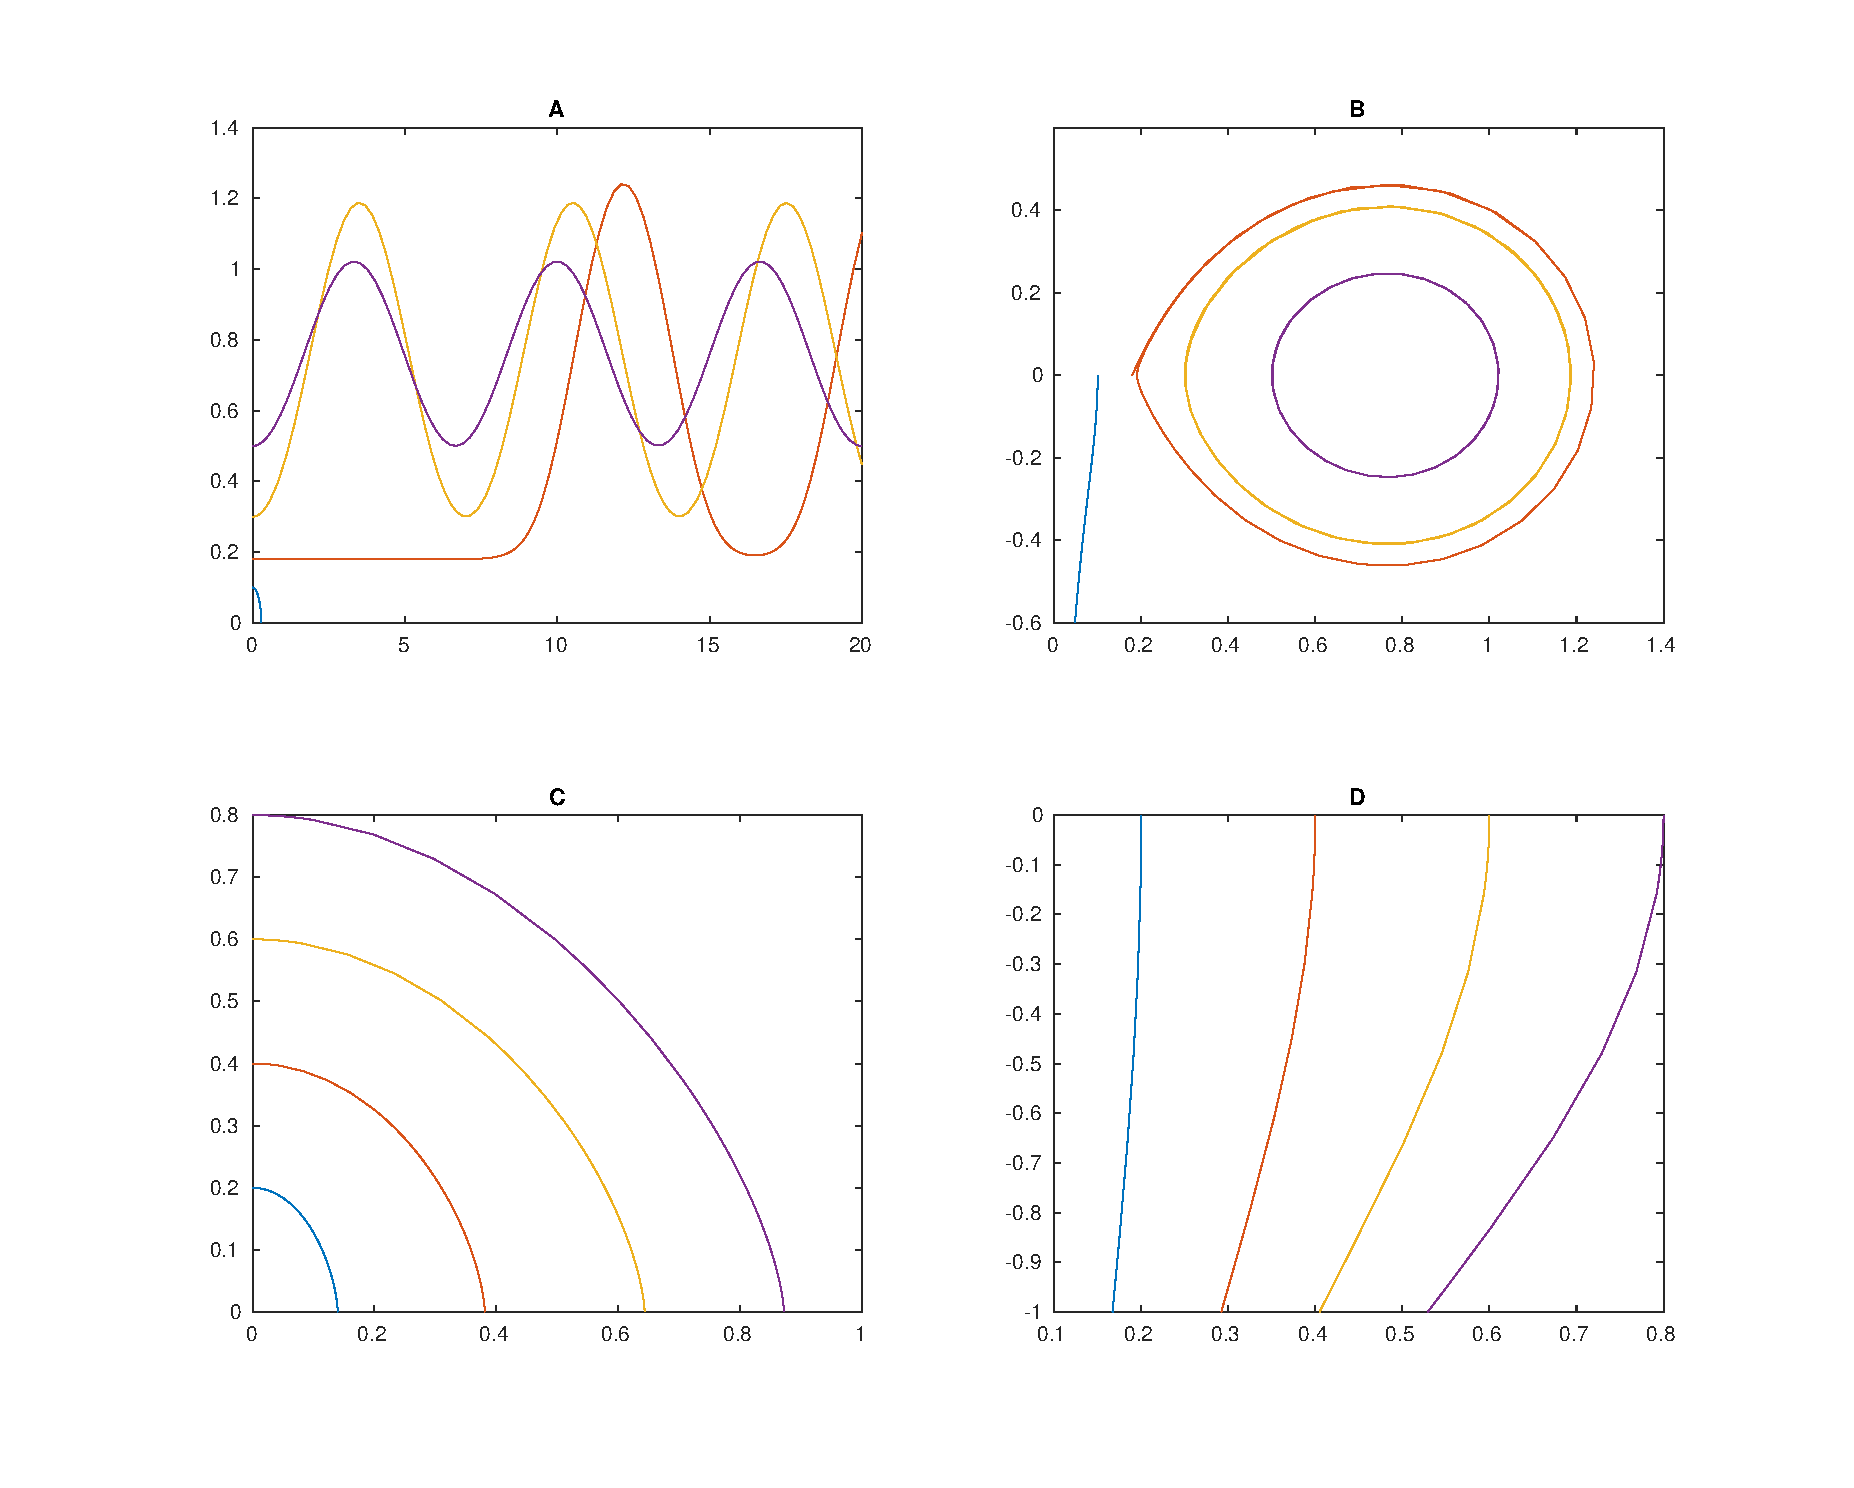
\includegraphics[width=\linewidth]{figures/quadplot_phaseplane_versus_time_2}
    \caption{
        A comparison of plots in the traditional distance-time representation compared to in the phase portrait.
        The left column (A and C) illustrates curves as displacement against time, while the right column (B and D) draw the same plots as shown in the respective figure to the left.
        Figures in different rows show the model under different initial conditions and parameters.
        Figures A and B show the displacement $b$ with starting positions $b=0.1,~b_1,~0.3,~0.5$,
        where $b_1$ is close to the first critical point of $f$. The parameters of Equation \ref{eqn:master} are $\mu=1,~q=0.2$.
        Figures C and D are instead computed with $\mu=1,~q=1$ with $b$ taking initial values $0.2,~0.4,~0.6,~0.8$.
        In all figures, $b$ has zero initial starting velocity.
    }
    \label{fig:phaseportrait_compare}
\end{figure}
Oscillations are represented in the phase-plane as closed loops.
It becomes easier to see the critical points,
namely the stationary point in the centre of the closed loops,
and the inflection point between the regions of closure and oscillation.
See Figure \ref{fig:phaseportrait_compare} for a demonstration.
The most common form of the phase portrait representation that we will observe in this problem is shown in subfigure B from Figure \ref{fig:phaseportrait_compare}.
Within a bounded region of $b$, closed oscillations occur,
and outside of this we experience eventual closure.

Recall Equation \ref{eqn:master}, of the form $d^2b/dt^2 = f(b)$.
Assume the right hand side $f(b)$ is the derivative (with respect to $b$, remaining aware that $b$ depends on $t$) of some function $F(b)$.
Remaining aware that $b$ is a function itself of $t$, we have
\begin{equation}
    \frac{d}{db}F(b) = f(b),
\end{equation}
and if we differentiate with respect to $t$ instead, we obtain
\begin{equation}
    \frac{d}{dt}F(b) = \frac{dF}{db}\frac{db}{dt} = f(b)\frac{db}{dt}.
\end{equation}
From Equation \ref{eqn:master}, we find, on multiplying both sides by $db/dt$ and finding antiderivatives,
\begin{align}
    \frac{d^2b}{dt^2} \frac{db}{dt}                                   & = f(b) \frac{db}{dt} \\
    \Rightarrow \frac{1}{2}\frac{d}{dt}\left( \frac{db}{dt} \right)^2 & = \frac{d}{dt}F(b).
\end{align}
Integrate both sides and we obtain a result that resembles an expression for kinetic energy, namely,
\begin{equation}
    \frac{1}{2}\left(\frac{db}{dt}\right)^2 = F(b) + C,
    \label{eqn:integral_kinetic_energy}
\end{equation}
with constant of integration $C$. Variation of this constant leads to a family of solutions.
Extremely important to note is that we have an equation in terms of $\frac{db}{dt}$ and $b$, which are the vectors defining the phase portrait.
Hence the curves that appear in the phase portrait represent all the curves that appear for different $+C$.

%figure with the $P(b)$ curves matched to phase portrait curves, namely y = F(x) against 1/2 y^2 = F(x)

Notice that Equation \ref{eqn:integral_kinetic_energy} is of exactly the same form as Equation \ref{eqn:first_order_reduction},
which we derived earlier.
Both expressions represent families of curves in the phase-portrait.
However, when reducing and solving the ODE to derive the first order reduction, we made the assumption of separability of variables,
which is not true in all cases,
whereas here we have covered a different method.
In combination of results, we will define the function $F$ as
\begin{equation}
    F(b) = (1-q)b - \frac{1}{2}b^2 + \frac{\mu q^2}{2b}
    \label{eqn:integral_curve_supposed}
\end{equation}
which is not necessarily a consistent result, as discussed in the derivation, but we will use this for verification.

We can use the plots of curves defined by Equations \ref{eqn:first_order_reduction} and \ref{eqn:integral_kinetic_energy} to inspect curves in the phase portrait.
For example, we can find the particular constants $C$ such that we generate the behaviours at the critical points.

%big section here on how we can analyse the plots and zeroes of the KE curves, in order to find the requirements on f for oscillations to occur

Oscillations occur when, for some $C$, the curve $\left((db/dt)^2\right)/2 = F(b) + C$ exhibits a closed loop.
It is necessary and sufficient for there to exist a region of inflection (an interval where the derivative is positive,
elsewhere negative) in $F(b)$ in order for this to occur.
This is equivalent to the requirement that $f(b)$ is somewhere positive.

Interesting behaviour occurs when the local minimum or maximum of $F(b)$ is a zero.
We want to investigate the integral curves to find the conditions required for
\begin{equation}
	F(b) + C = 0.
	\label{eqn:integral_curves_zeroes}
\end{equation}
If $\mu, q$ satisfy the condition for oscillations to occur,
it is evident that there exists a $C$ such that Equation \ref{eqn:integral_curves_zeroes} will have exactly two zeroes.
The interval between these is the region in which we observe the largest oscillation.

\subsection{The Jacobian matrix}

Recall the reduction of Equation \ref{eqn:master} to a first order system in Equation \ref{eqn:first_order_reduction}.
Using the function $f(b)$ which we have defined, the equation can be represented by a first order system as
\begin{align}
    \frac{\mathrm{d}b}{\mathrm{d}t} &= \hat{b} \\
    \frac{\mathrm{d}\hat{b}}{\mathrm{d}t} & = f(b)
    \label{eqn:first_order_modified}
\end{align}
We can construct an approximation for the function $f(b)$ about a point $b_0$ using the Taylor series expansion, assuming differentiability on the variable $b$, of the form
\begin{equation}
    f(b) = f(b_0) + (b-b_0)f'(b_0) + \frac{(b-b_0)^2 f''(b_0)}{2!} + \mathellipsis = \sum_{k=0}^\infty\frac{(b-b_0)^{k}f^{(k)}(b_0)}{k!}
    \label{eqn:taylor_series}
\end{equation}
Recall that $f(b)$ has zeroes. If we pick $b_0$ to be a zero of the function, then as $b\rightarrow b_0$,
we can simplify the Taylor series expansion.
More precisely, since $b_0$ is a zero of $f$, the $f(b_0)$ term tends to zero.
We keep the $(b-b_0)f'(b_0)$ since, while $b-b_0$ is small,
the terms succeeding it are far smaller in magnitude.
With the Taylor series applied, propose the approximation about a point $b_0$
\begin{align}
    \frac{db}{dt}       & = \hat{b}         \\
    \frac{d\hat{b}}{dt} & = (b-b_0)f'(b_0).
    \label{eqn:first_order_approximated}
\end{align}
Notice that this approximation is a linear system. The obtained approximation models the ODE $b''(t) = (b-b_0)(\mu q^2/b_0^3-1)$.
It is only valid local to points $b_0$ which are zeroes of $f$, so if $b-b_0$ grows in magnitude it is not sufficient.
If we suppose a substitution of the form
\begin{align}
    X & = b - b_0  \\
    Y & = \hat{b},
\end{align}
then $X$ represents the vicinity of $b$ to $b_0$, which is small,
and $Y$ is a straight substitution of the velocity value $\dot{b}$.
We can rewrite the linear system again, this time using our substituted values
\begin{align}
    \frac{dX}{dt} & = \frac{d}{dt}\left(b-b_0\right) = \hat{b} \\
    \frac{dY}{dt} & = \frac{d}{dt}\hat{b} = (b-b_0)f'(b_0)
\end{align}
which can be expressed as the matrix equation
\begin{equation}
    \frac{d}{dt}\begin{pmatrix}
        X \\
        Y
    \end{pmatrix} = \begin{bmatrix}
        0      & 1 \\
        f'(b_0) & 0
    \end{bmatrix} \begin{pmatrix}
        X \\
        Y
    \end{pmatrix}.
    \label{eqn:first_order_approximated_substituted_matrix}
\end{equation}
This is the Jacobian matrix for the ODE. The linearisation is of the form
\begin{align*}
    \frac{\mathrm{d}X}{\mathrm{d}t} &= g_1(X,Y) = Y \\
    \frac{\mathrm{d}Y}{\mathrm{d}t} &= g_2(X,Y) = Xf'(b_0) 
\end{align*}
to represent the linear approximation of the ODE at an equilibrium \(b_0\).
Then the Jacobian is the matrix of first order derivatives of $X$ and $Y$,
\begin{equation}
    \begin{bmatrix}
        \frac{\partial g_1}{\partial X}(b_0) & \frac{\partial g_1}{\partial Y}(b_0) \\
        \frac{\partial g_2}{\partial X}(b_0) & \frac{\partial g_2}{\partial Y}(b_0) 
    \end{bmatrix} = \begin{bmatrix}
        0 & 1 \\
        f'(b_0) & 0
    \end{bmatrix},
\end{equation}
which matches Equation \ref{eqn:first_order_approximated_substituted_matrix}.
The characteristic polynomial for this matrix is
\begin{equation}
	\lambda^2 - f'(b_0) = 0.
	\label{eqn:onemass_char_poly}
\end{equation}
We have obtained the Jacobian matrix identical to how it was defined in our introduction,
however the problem itself is simplified from the general form we first covered.

% discuss the implications of this analysis and the matrix eigenvectors

\section{Computational results and further analysis}

\subsection{Formulating the problem for MATLAB}

%providing an input for MATLAB
We use MATLAB, primarily the \texttt{ode45()} function, to compute solutions numerically.
However, the governing differential equations must be provided as a first order system.
We have explored first order forms of Equation \ref{eqn:master} earlier,
in Equations \ref{eqn:first_order_system} and \ref{eqn:vector_system}.
MATLAB performs a time stepping method on a first order vector valued ODE,
which is given in out case as
\begin{equation*}
	\frac{d}{dt}\begin{pmatrix}
		b \\
		\hat{b}
	\end{pmatrix} = \begin{pmatrix}
		\hat{b} \\
		f(b)	
	\end{pmatrix}
\end{equation*}
By using \texttt{ode45}, MATLAB performs numerical integration on all the equations in the system,
thus giving numerical solutions for $b$ and $\dot{b}$ in terms of time $t$, subject to initial conditions.
In most cases, we will consider the plate moving from rest ($\hat{b}(t=0) = 0$) given an initial position $b=b_0$.
All scripts are available in the appendix of this report.

\subsection{MATLAB results and inspection}

\begin{figure}[h!]
    \centering
    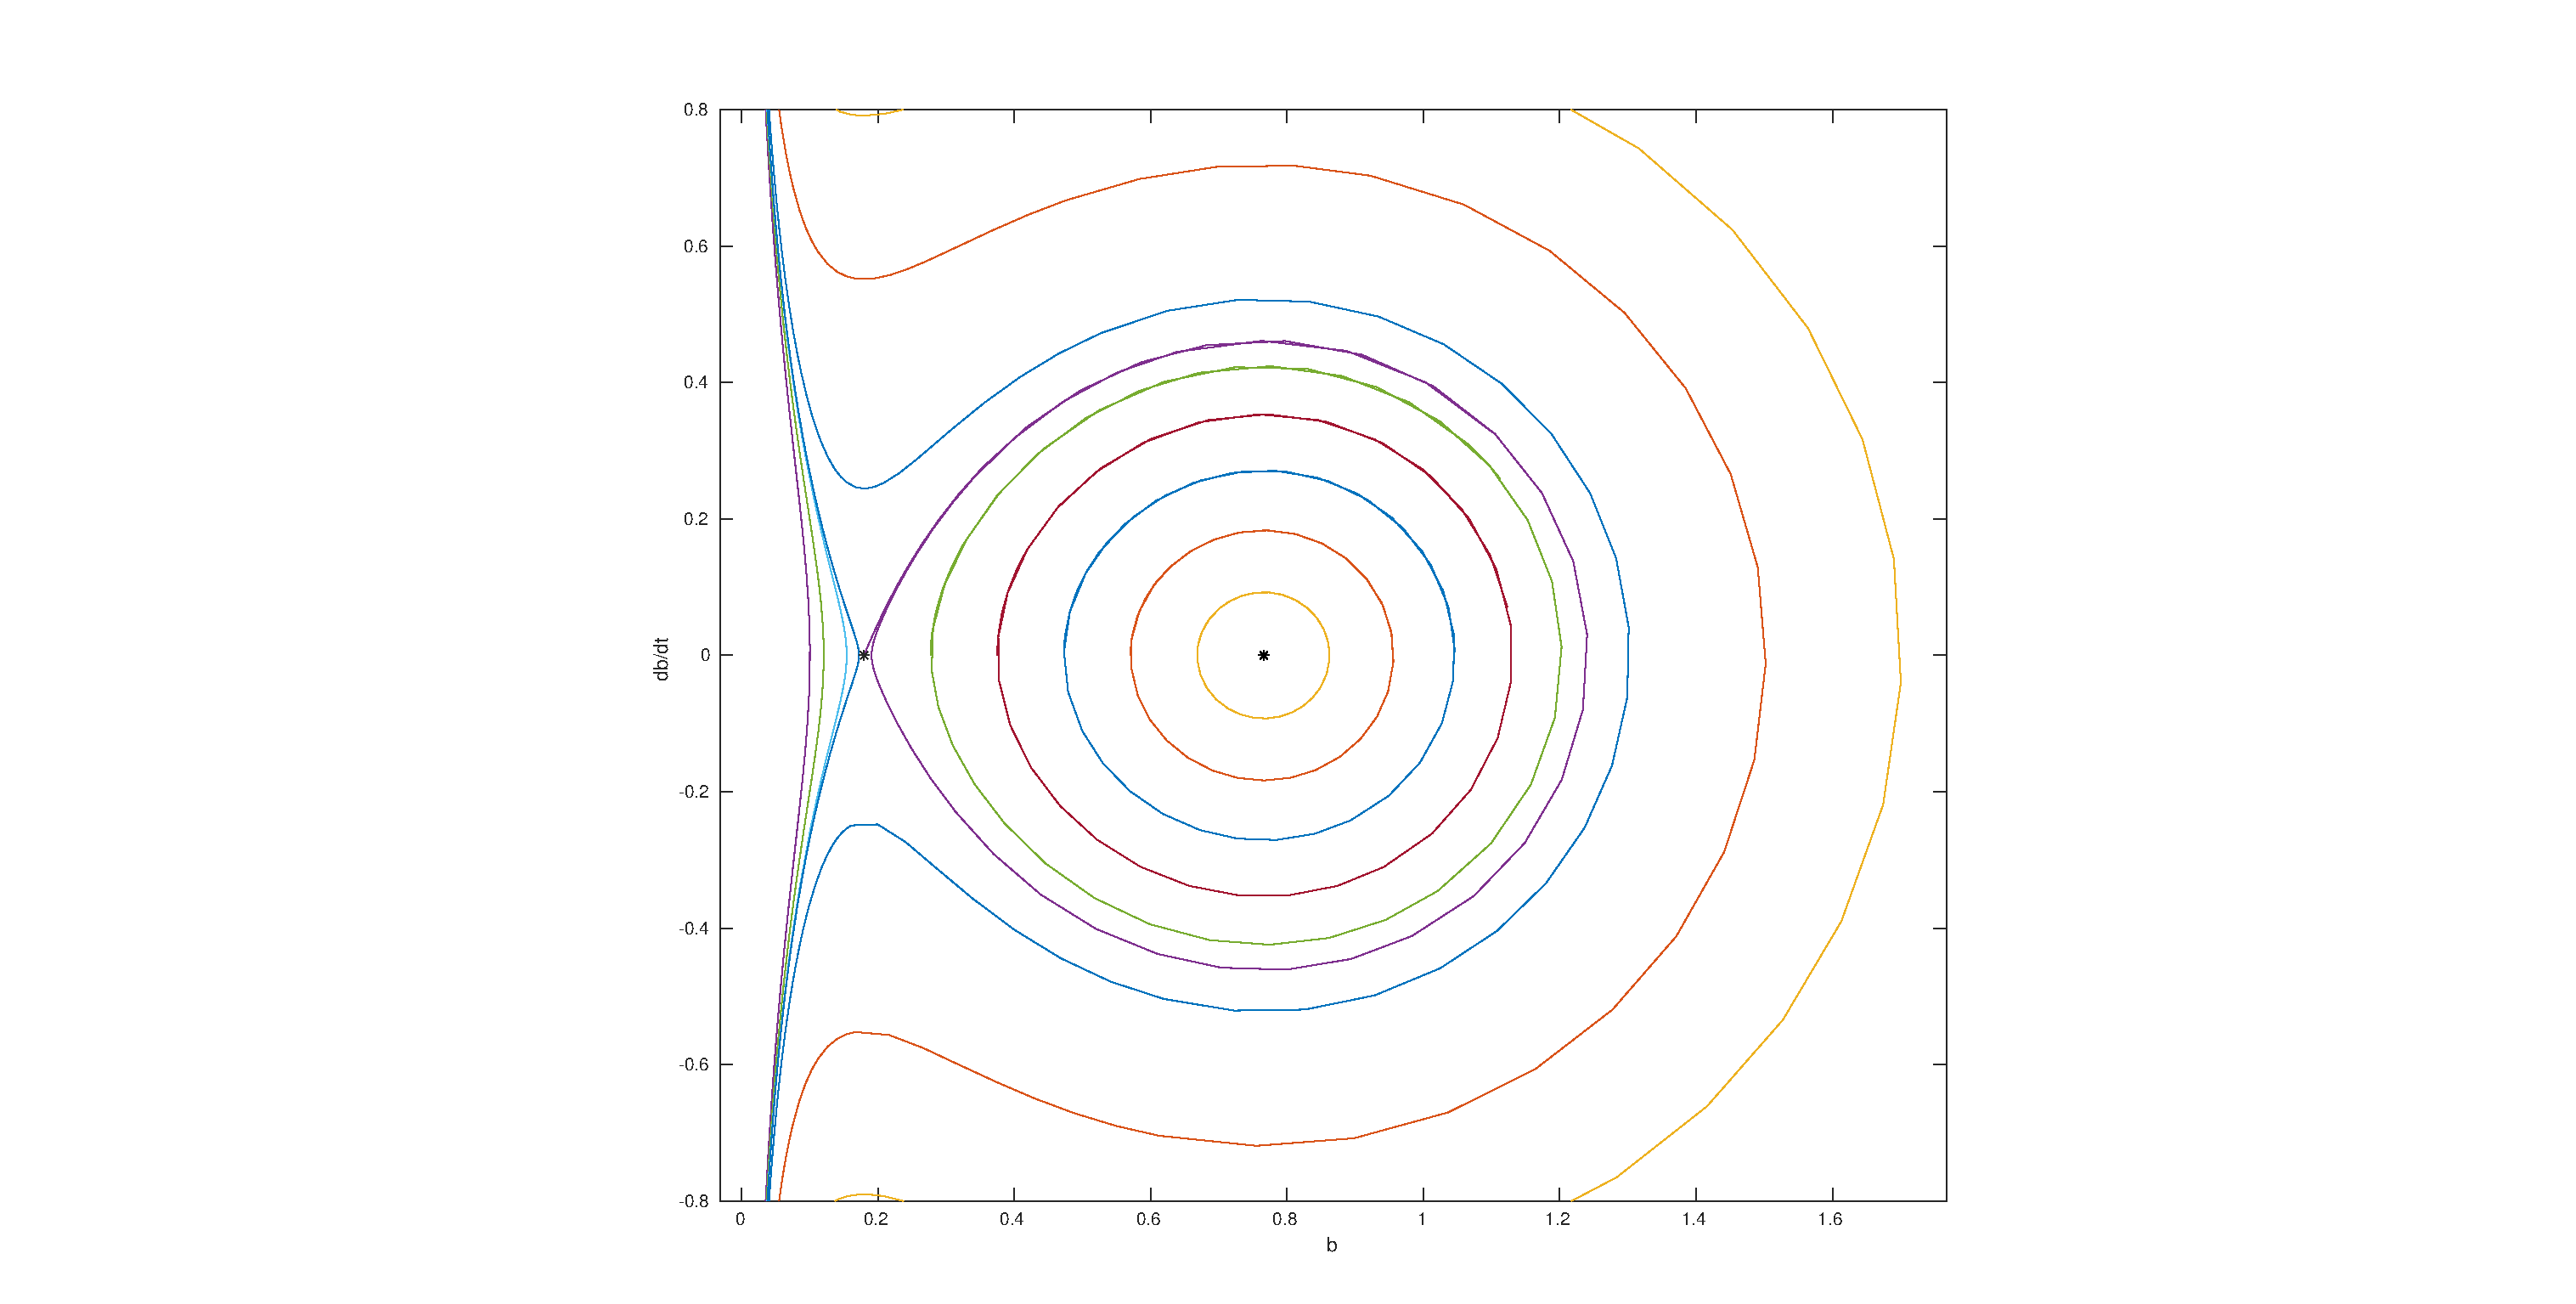
\includegraphics[width=\linewidth]{figures/phaseportrait}
    \caption{
        Representation of all families of curves in the phase portrait representation of numerical solutions for Equation \ref{eqn:master}.
        The parameters are set with $\mu = 1,~q=0.2$. The critical points were computed to be $b_1 \approx 0.1795,~ b_2 \approx 0.7659$, and have been marked.
    }
    \label{fig:phaseportrait_oscillations}
\end{figure}

\begin{figure}[h!]
    \centering
    \includegraphics[width = 0.7\linewidth]{figures/stable_oscillations.eps}
    \caption{
        Oscillations about the equilibrium solution $b_2$ with parameters $\mu=1,~q=0.1$, represented in the phase portrait.
        Computed using a random angle and small modulus to offset initial conditions within a small disc about $b_2$ in the phase-plane.
        We always observe regular oscillations that continue indefinitely.
    }
    \label{fig:stable_oscillations}
\end{figure}

\begin{figure}[h!]
    \centering
    \includegraphics[width=\linewidth]{figures/trajectories_unstable.eps}
    \caption{
        Trajectories about the equilibrium solution $b_1$ with parameters $\mu=1,~q=0.1,$ drawn in the phase portrait.
        Paths either accelerate to closure (left of the fixed point), fall into orbit about $b_2$ (right),
        or follow a path outside of the closed region of oscillations (top and bottom) before closure.
        We view an extremely close image of the unstable point,
        showing how oscillations (right of the stationary point) come extremely close to the equilibrium.
    }
    \label{fig:unstable_trajectories}
\end{figure}
We will first consider a range of behaviours exhibited by the model with the fixed parameters $\mu=1, q=0.2$,
as used in sufigures A and B of Figure \ref{fig:phaseportrait_compare}.
Figure \ref{fig:phaseportrait_oscillations} is a plot showing all families of curves in the phase plane for these parameters.

We can see there are four types of curve represented.
Curves that cross the horizontal axis to the left of the point $b_1$ represent the plate travelling and accelerating (negative velocity as the plate travels in the non-positive direction) immediately to closure.
Closed loops within the enclosed region are oscillations that continue indefinitely.
Curves to the right of the closed loops represent the plate also travelling towards closure,
but undergoing a period of deceleration close to the critical value.
This leaves two others. Two separate curves emerge directly from the point $b_1$ itself,
however the computation is incapable of computing this path exactly when we start at zero.
If we start at $b_1+\epsilon$ where $\epsilon$ is small,
the solution fails to form a closed loop that returns to its start,
due to the precise behaviour of the ODE close to this critical point being subject to numerical error.
Instead, this loop is shown to slightly increment the return position positively when an oscillation has been completed.
The stationary point at $b_2$ is the oscillation with no energy,
which is similar to the other closed loops.
\begin{figure}[h!]
    \centering
    \includegraphics[width=\linewidth]{figures/equilibrium_solutions_eigenvalues_too.eps}
    \caption{
        Equilibrium solutions (left) of $f$ for fixed $\mu=1$ as $q$ changes, and eigenvalues of the Jacobian matrix (right) as the solutions change.
        The eigenvalues in the right figures are always pairs up to sign, since the equation involves the determinant of the \(2\times 2\) Jacobian matrix.
        The eigenvalues of $b_1$ are always entirely real, while the eigenvalues of $b_2$ are always entirely imaginary.
        Ellipsoids are rendered to mark the moduli of the eigenvalues for different values of $q$.
    }
    \label{fig:equilibrium_eigenvalues}
\end{figure}

We will compute eigenvalues of the equilibria with data to four significant figures, taking \(b_1 = 0.1795\) and \(b_2 = 0.7659\).
We are interested in the eigenvalues of \ref{eqn:first_order_approximated_substituted_matrix}.
An eigenvalue of the Jacobian is determined by the characteristic polynomial which we saw in Equation \ref{eqn:onemass_char_poly}.
At \(b_1\) we have roots at \(\lambda = \pm 2.4371\), which are entirely real,
and at \(b_2\) we have roots at \(\lambda = \pm 0.9544 i\), which are entirely imaginary.
Due to one eigenvalue of \(b_1\) having positive real part,
we can deduce that $b_1$ is an unstable equilibrium in this case.
Figure \ref{fig:equilibrium_eigenvalues} shows the equilibrium solutions as the parameter $q$ changes and plots their eigenvalues in the complex plane as the equilibrium solutions converge.

In the proximity of $b_2$, oscillations can be observed about the fixed point,
but in proximity to $b_1$ we can observe a variety of behaviours. 
Figures \ref{fig:stable_oscillations} and \ref{fig:unstable_trajectories} show the behaviours local to each equilibrium solution.
We conclude that if the Jacobian has entirely real eigenvalues at a stationary point, it is unstable,
whereas if the eigenvalues are entirely imaginary (complex with zero real part) then it is stable. 

Clearly in order for a stationary point \(b_0\) to have real eigenvalues, we must have \(f'(b_0) \ge 0\) such that the characteristic polynomial has real roots.
If \(f'(b_0)=0\), eigenvalues will be zero since $\mathbf{J}$ is not a full-rank matrix.
This condition can be expanded and written more explicitly as \(\mu q^2 \ge b_0^3\), which is a surprisingly simple expression.

In any case where the curve $f$ has exactly two zeroes for positive $b$,
we can compute these points and the eigenvalues of the Jacobian at each.
If the curve $f$ has, instead, exactly one zero for positive $b$,
then the curve $F(b)$ has a point of inflection, but its gradient ($f$ itself, by definition) is always negative.
We require equality in Equation \ref{eqn:osc_condition} for any suitable parameters, which can be rearranged into the form
\begin{equation}
    27\mu q^2 = 8(1-q)^3.
\end{equation}
We have no restrictions on uniqueness of solutions to this equation. Suitable real rational values for $\mu, q$ are \(\mu = 64/81, q=1/3\).
Real rational solutions allow us to solve this case analytically.
The single equilibrium is $b_0=(\mu q^2)^{1/3} = 2^2/3^{5/3}$. We can solve the eigenvalue equation as follows
\begin{align*}
    &\det \left(\mathbf{J} - \lambda \mathbf{I}\right) = 0 \\
    &\lambda ^2 - f'(b_0) = 0 \\
    &\lambda ^2 - f'((\mu q^2)^\frac{1}{3}) = 0 \\
    &\lambda ^2 + 1 - \frac{\mu q^2}{(\mu q^2)^\frac{1}{3}} = 0 \\
    &\lambda ^2 + 1 - (\mu q^2)^\frac{2}{3} = 0 \\
    &\lambda ^2 + 1 - \frac{2^4}{3^\frac{10}{3}} = 0 \\
    &\lambda ^2 = \frac{2^4}{3^\frac{10}{3}} - 1 \\
    &\lambda = \pm \sqrt{ \frac{2^4}{3^\frac{10}{3}} - 1 } \\
    &\lambda \approx \pm 0.7675i
\end{align*}
hence at the single equilibrium, the eigenvalues are entirely imaginary, similar to the $b_2$ equilibrium in the particular case we computed earlier.

\subsection{Comparison to analytical results}

\begin{figure}[h!]
    \centering
    \includegraphics[width=\linewidth]{figures/sqrt_integral_curves.eps}
    \caption{
        Plots of $F(b)+C$ and $\sqrt{F(b)+C}$ against $b$.
        The right-hand-side plot resembles the plots of the model's behaviour in the phase portrait,
        since Equation \ref{eqn:integral_kinetic_energy} gives us a relationship between the two.
    }
    \label{fig:sqrt_curves}
\end{figure}
The region of inital $b$, with zero initial velocity, for which oscillations will occur,
is computed to be the approximate interval $(0.18,1.24)$.
We will assume Equation \ref{eqn:integral_curve_supposed}.
If the integration constant satisfies $C = -F(b_1)$,
then the curve has exactly two positive zeroes:
one being at $b=b_1$ and the other where $b>b_2$ as the curve crosses the horizontal axis as it tends to negative infinity.
This means the curve \(F(b)\) is also zero at the stationary point \(b = b_1\).
Hence the range of zeroes to verify results should be the solutions to the equation $F(b)-F(b_1)=0$, in full
\begin{equation}
    (1-q)b - \frac{1}{2}b^2 + \frac{\mu q^2}{2b} - F(b_1) = 0.
    \label{eqn:integral_curves_zeroes_explicit}
\end{equation}
This is guaranteed to be zero at $b_1 \approx 0.1795$.
We have the parameters \(\mu = 1,~ q = 0.2\)

We are more interested in whether or not the other end point of the interval is consistent.
The function \(F(b) + C\) draws curves in the phase portrait.
We want to consider oscillations, which require solutions to the equation
\begin{equation}
    F(b) + C = (1-q)b - \frac{1}{2}b^2 + \frac{\mu q^2}{2b} + C = 0.
\end{equation}
It is fairly simple to figure out that if \(F(b)+C=0\) is required at the stationary point \(b_1\),
then \(C = -F(b_1)\)
The function \(F(b)-F(b_i)\) is zero at $b_i$, allowing us to construct functions representing the kinetic energies of a solution to the ODE,
which take zero at the equilibrium solutions.

Figure \ref{fig:sqrt_curves} shows plots of $F(b)+C$ and $\sqrt{F(b)+C}$ for different constants $C$.
The blue curve is the line $F(b)-F(b_1)$ at the stationary point $b_1$,
and plotting its square root forms a sharp point where it intersects with the horizontal axis.
This resembles the shape of the unstable equilibrium in the phase portrait,
which we visualised in Figure \ref{fig:unstable_trajectories}.

We will now rigorously show that Equation \ref{eqn:osc_condition} guarantees oscillations.
Assume that $f(b)$ is somewhere strictly positive, which is equivalent to \ref{eqn:osc_condition}.
We do not include the case of equality,
which is where $f(b)$ is zero exactly once.
Equivalently, $F(b)$ has a region of inflection,
since its gradient $f(b)$ is positive on a given interval.
As shown by Figure \ref{fig:sqrt_curves},
the curve $F(b)-F(b_1)$ is equivalent to the closed loop in the phase portrait that starts and ends at $b_1$.
Curves $F(b)-F(b_1)-\eta$, where $\eta$ is small,
correspond to closed loops bounded by the curve $F(b)-F(b_1)$.
For sufficiently small $\eta$ such that $b_1+\eta$ is contained between the zeroes of $F(b)-F(b_1)$,
we have a closed loop, which corresponds to an orbit represented in the phase portrait.

\section{Review and motivation}

The single mass model is capable of producing oscillations within a bounded region.
Trajectories converge towards the vicinity of the unstable equilibrium when they pass near the boundary for oscillations.
Close to the stable equilibrium, oscillations are periodic and regular.
However, the motions of the mass have a very simple pattern which do not relate very strongly to the complicated nature of the mechanics of phonation.
We will develop a two mass model, using the concepts we have introduced so far, for a further study.

% derivation of the conditions on +C which guarantee the closed orbit. 

% rigorous understanding of the range of oscillations

% behaviour of oscillations local to the "matrix points", tie in the analysis to the matrix methods.

% comparison of phaseplane and distance-time graphs




%\bibliographystyle{unsrt}
%\bibliography{sources}

%\end{document}